% Spring Mass system in TikZ: Short Drawing Guide
% Latexdraw.com
% 26/04/2021, 16:45

\documentclass[border=0.2cm]{standalone}

% Required package and libraries
\usepackage{tikz}
\usetikzlibrary{decorations.pathmorphing,patterns}

\begin{document}
	
	
	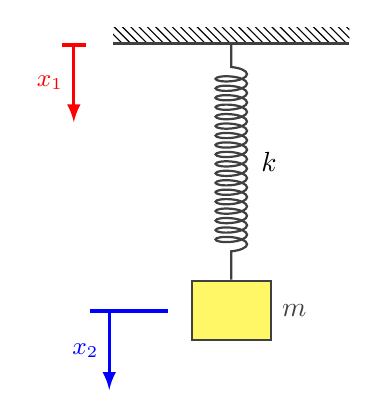
\begin{tikzpicture}[black!75,thick]
		
		% Supporting structure
		\fill [pattern = north west lines] (-1.5,0) rectangle ++(3,.2);
		\draw[thick] (-1.5,0) -- ++(3,0);
		
		% Spring 
		\draw
		[
		decoration={
			coil,
			aspect=0.3, 
			segment length=1.2mm, 
			amplitude=2mm, 
			pre length=3mm,
			post length=3mm},
		decorate
		] (0,0) -- ++(0,-3) 
		node[midway,right=0.25cm,black]{$k$}; 
		
		% Mass
		\node[draw,
		fill=yellow!60,
		minimum width=1cm,
		minimum height=0.75cm,
		anchor=north,
		label=east:$m$] at (0,-3) {};
		
		% x1 arrow
		\draw[very thick,
		red,
		|-latex] (-2,0) -- ++(0,-1)
		node[midway,left]{\small $x_1$};
		
		% x2 arrow
		\draw [very thick,
		blue,
		-latex
		] (-0.8,-3.4) -- ++(-1,0) ++(0.25,0) -- ++ (0,-1)
		node[midway,left]{\small $x_2$};
		
	\end{tikzpicture}
	
\end{document}